\section{Planning}
\SectionPage

\begin{frame}
  \frametitle{Features}
  \begin{itemize}
    \item Easy to extend (with modules)
      \begin{itemize}
        \item Low bar to create a module
        \item Easy to reason about how modules work together
      \end{itemize}
    \item Proto-modules should extend the application to include these features:
      \begin{itemize}
        \item Can open, edit, delete files
        \item Has LSP support
        \item Can compile and execute a program
      \end{itemize}
  \end{itemize}
\end{frame}

\begin{frame}
  \frametitle{Goals}
  % TODO: Should probably make these points more concrete
  \begin{itemize}
    \item Should be better than the current IDE
      \begin{itemize}
        \item Easy installation
      \end{itemize}
    \item Easy for the next \sout{sucker} developer to change core functionality
    \item Have a good module developer experience
  \end{itemize}
\end{frame}

\begin{frame}
  \frametitle{What Is A Module?}
  \begin{itemize}
    \item Third Party Code to be executed/interpereted
      \begin{itemize}
        \item Tailormade Scripting Language
        \item An already existing programming language
      \end{itemize}
  \end{itemize}
\end{frame}

\begin{frame}
  \frametitle{Granularity}
  \begin{itemize}
    \item How \textit{big} is a module?
    \begin{itemize}
      \item Could create an IDE module which does everything
      \begin{itemize}
        \item Not very granular
      \end{itemize}
      \item Could create a module for each function
      \begin{itemize}
        \item Very granular
      \end{itemize}
    \end{itemize}
  \end{itemize}
\end{frame}

\begin{frame}
  \frametitle{Module Family}
  \begin{itemize}
    \item Grouping of related modules that work together.
    \item Example
    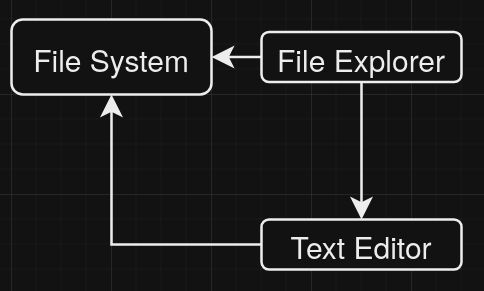
\includegraphics[width=0.9\textwidth]{./pics/ide-family.png}
  \end{itemize}
\end{frame}

\section{Modeling a Module}
\SectionPage

\begin{frame}
  \frametitle{How To model A Module?}
  \begin{itemize}
    \item A module needs to:
      \begin{itemize}
        \item Initialize some state
        \item Update the state based on events
        \item Render the view based on the state
      \end{itemize}
    \item Module architecture is inspired by Elm and MVC
    \item A module should be \textit{pure}
  \end{itemize}
\end{frame}

\begin{frame}
  \frametitle{Module V.1}
  \begin{itemize}
    \item First plan
    \begin{enumerate}
      \item Create an IDE
      \item Extend the IDE, to allow for a module architecture
      \item Modules call the application using some DSL
    \end{enumerate}
    \item Pros
    \begin{itemize}
      \item \textit{Easy} to implement
      \item Get a good understanding of what features might be needed
    \end{itemize}
    \item Cons
    \begin{itemize}
      \item Not really modular
      \item Will be subpar compared to existing software
    \end{itemize}
  \end{itemize}
\end{frame}

\begin{frame}
  \frametitle{Module V.1 - Final}
  \begin{itemize}
    \item Second plan
    \begin{itemize}
      \item A module exposes three functions, that are invoked by the core
      \begin{itemize}
        \item Init - Returns a set of fields, which are added to the core state
        \item Update - Returns a set of fields which are updated
        \item View - Returns a set which represents HTML, which is rendered by
          the Core
      \end{itemize}
      \item Pros
      \begin{itemize}
        \item Easy to keep modules pure
        \item Optimalization is possible due to the pureness of modules
        \item Easy to reason about module cooperation
      \end{itemize}
      \item Cons
      \begin{itemize}
        \item State is append-only
        \item State can only grow
        \item Not really modular
      \end{itemize}
    \end{itemize}
  \end{itemize}
\end{frame}

\begin{frame}
  \frametitle{Example}
  TODO: Add example
\end{frame}

\begin{frame}
  \frametitle{Module V.1 - Final.Final}
  \begin{itemize}
    \item Third, and hopefully the final plan
      \begin{itemize}
        \item Init - Returns a set of modifications
      \end{itemize}
    \item Pros
    \begin{itemize}
      \item Modular
      \item Modules can \textit{invoke} other modules
    \end{itemize}
    \item Cons
    \begin{itemize}
      \item Complex to implement
    \end{itemize}
  \end{itemize}
\end{frame}

\begin{frame}
  \frametitle{Example}
  TODO: Add example
\end{frame}

\begin{frame}
  \frametitle{My hat is cooler than yours}
  \begin{itemize}
    \item The Developer, the main userbase
    \begin{itemize}
      \item Need plugins to have \textit{any} experience
    \end{itemize}
    \item The Module Developer, the secondary userbase
      \begin{itemize}
        \item Language Agnostic Module Architecture
        \item Good documentation and examples
        \item Should prioritize the Module Developer Experience
      \end{itemize}
    \item Maintainer Experience
      \begin{itemize}
        \item Good documentation
        \item Good testing
        % TODO: Unsure if I should mention this, as my CI/CD does not work, and
        % I am not sure if I am going to fix it
        \item CI\/CD
      \end{itemize}
  \end{itemize}
\end{frame}
